\section{核災應變機器人設計}

\subsection{Vision}
在核災中,我們必須辨識出該城市內之物品,找出可能的目標物品以及生還者。
由於此次人本專題我們使用了Duckietown城市模擬核災發生並作為驗證場地,所以重新組裝了一台Super Duckiebot。
在視覺部份因考量到車體大小,故選擇使用體積較小的Jetson Nano處理相關視覺運算,同時也使用運算量較小的MobileNet-SSD Model,
在影像辨識部份利用RGB資訊進行Training,精準度、輕巧度及靈敏度是Artifact search相當重要的指標,控制訓練後Model的大小將其放置於較輕巧的Jetson Nano上運行,並且考量到幀數(FPS)也就是一秒讀取幾張圖片進行辨識,各個環節環環相扣。

當變試出目標物後,隨即使用Depth資訊利用投影矩陣取得目標物與相機之距離,並與UWB Localization結合,最後呈現於Rviz上觀看。



\subsection{Localization}


\begin{figure}[t]
  \centering
    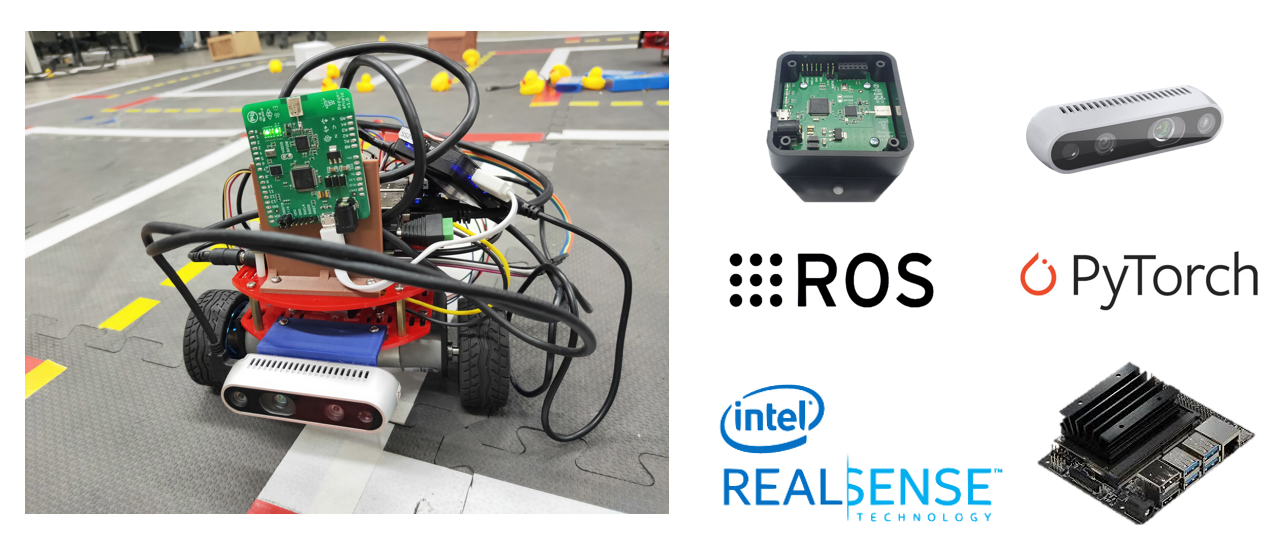
\includegraphics[width=\columnwidth]{images/car.png}
        \caption{車體設計及相關環境}
 \label{figure:car}
\end{figure}









